\subsection{Environmental Geometry and Workspace}

We consider the Rapidly-exploring Random Tree (RRT) path planning problem in a 2D configuration space $\mathcal{X} \subseteq \mathbb{R}^2$, where the free space is defined as $\mathcal{X}_{\text{free}} = \mathcal{X} \setminus \mathcal{X}_{\text{obs}}$. The workspace is bounded such that $\mathcal{X} = [x_{\min}, x_{\max}] \times [y_{\min}, y_{\max}] \subset \mathbb{R}^2$. The environment is characterized by $\mathcal{X}_{\text{obs}}$, which consists of clustered, maze-like obstacle structures represented as polygonal regions, enabling efficient collision checking via geometric intersection tests.

The objective is to incrementally grow a tree $\mathcal{T} = (V, E)$ from a start configuration $q_{\text{start}} \in \mathcal{X}_{\text{free}}$ toward a goal $q_{\text{goal}} \in \mathcal{X}_{\text{free}}$. The standard RRT algorithm samples configurations uniformly from $\mathcal{X}_{\text{free}}$ and expands the tree toward sampled points via a steering function with step size $\eta$, adding collision-free edges until the goal is reached within threshold $\epsilon$.

We focus on maze-like environments characterized by clustered obstacles, narrow passages, and dead ends. These environments pose significant challenges for path planning, requiring navigation through tight spaces and U-shaped, nested obstacles. We assume that $\mathcal{X}_{\text{free}}$ is connected, which guarantees that at least one collision-free path exists between $q_{\text{start}}$ and $q_{\text{goal}}$.

To generate these layouts, we use a grid-based random walk algorithm to define the maze topology. Although the underlying structure is determined by discrete grid cells (e.g., a $20 \times 20$ grid), the obstacles themselves are represented as rectangular Shapely objects within the continuous configuration space $\mathcal{X} \subseteq \mathbb{R}^2$. Consequently, while maze density is determined by the grid dimensions, the RRT algorithm samples directly from continuous space rather than being restricted to discrete cells.

\begin{figure}
    \centering
    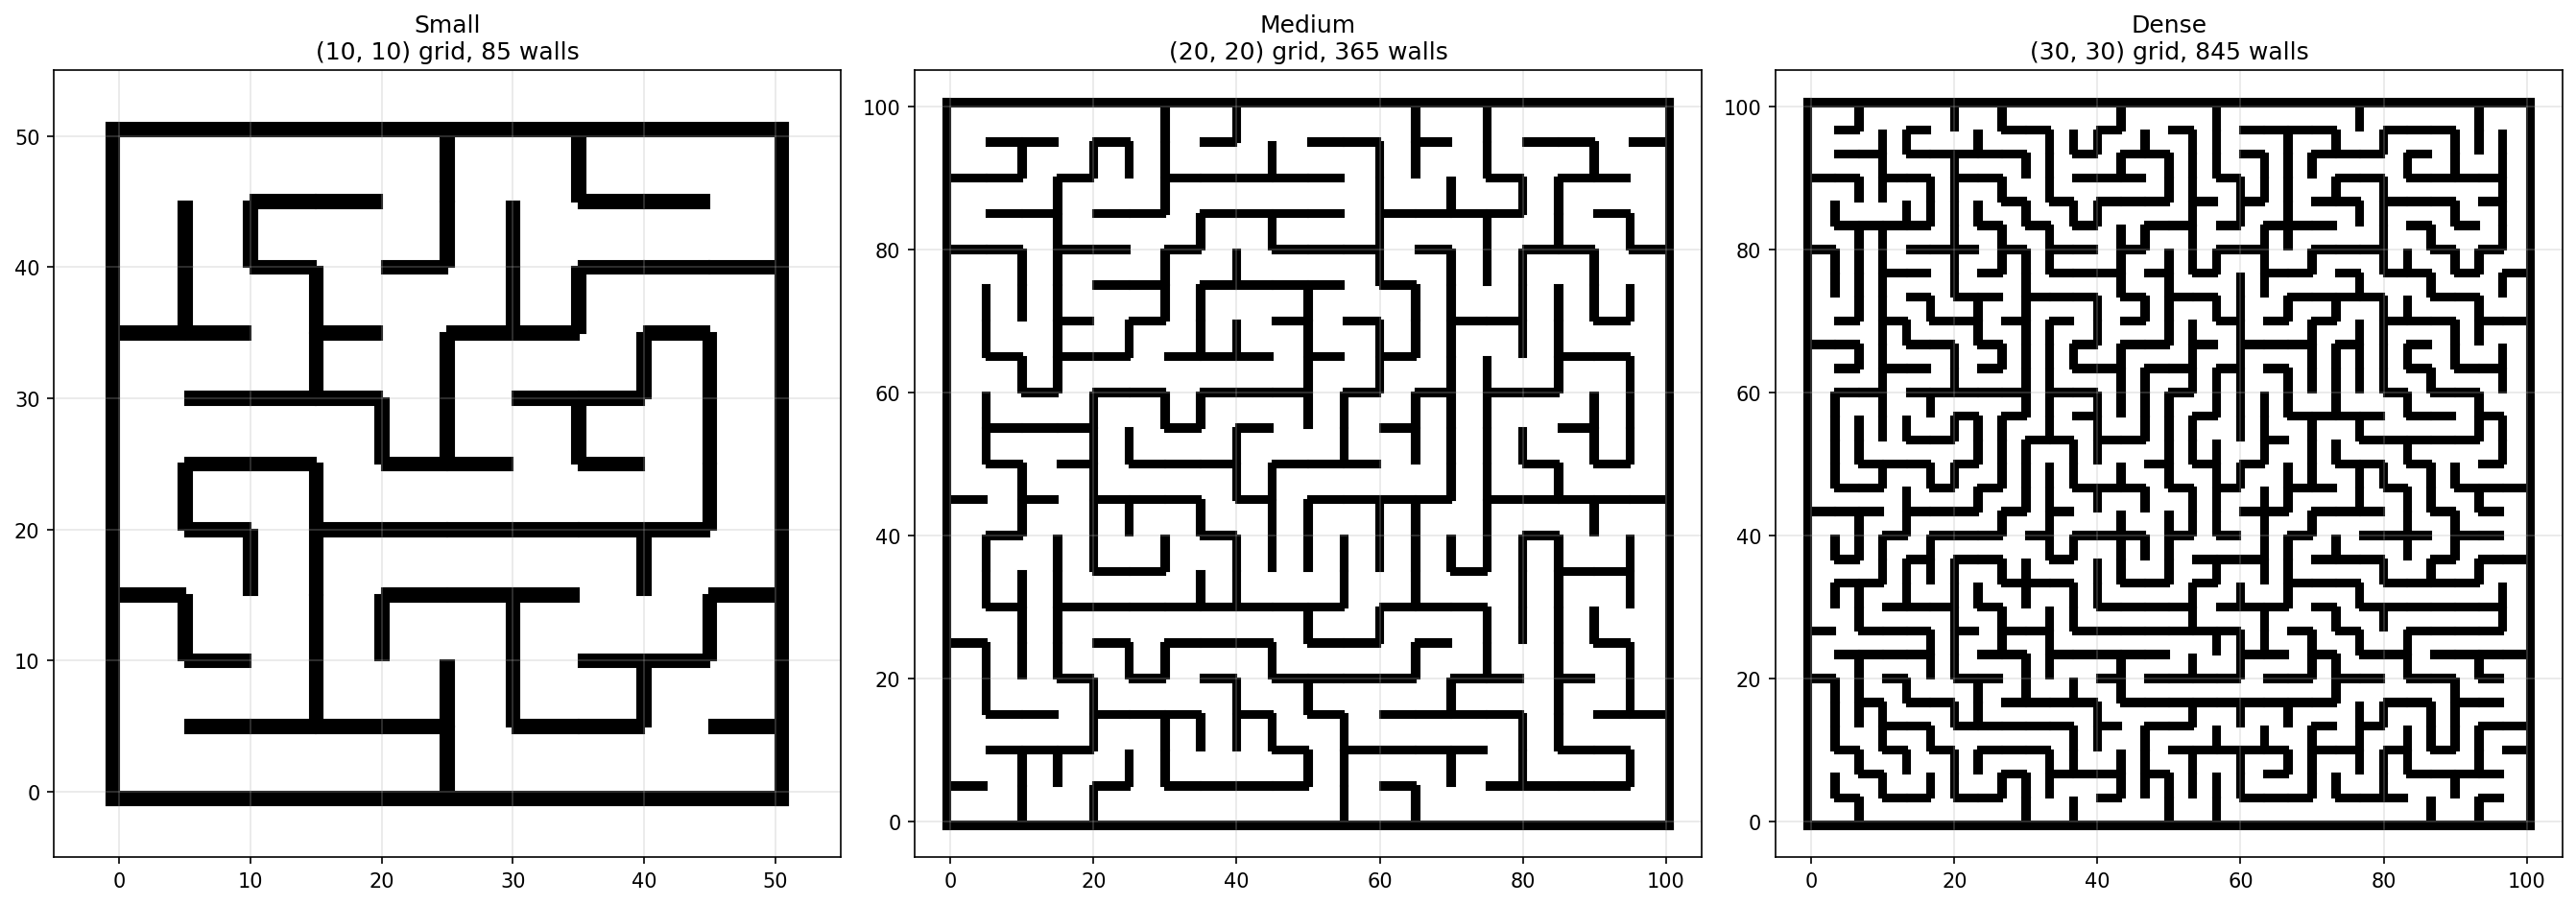
\includegraphics[width=1.00\linewidth]{maze_comparison.png}
    \caption{Example Configuration Spaces}
    \label{fig:placeholder}
\end{figure}

\subsection{Goal Uncertainty Representation}

We consider the problem where the goal location $q_{\text{goal}}$ is unknown and must be inferred from noisy sensor observations. The planner maintains a probabilistic belief about the goal location. This belief evolves throughout the navigation process as the planner receives new readings of the goal location.

We represent the goal belief as a multivariate Gaussian distribution:
\begin{equation}
    P(q_{\text{goal}} | \mathcal{Z}) = \mathcal{N}(\mu, \Sigma)
\end{equation}
where $\mu \in \mathbb{R}^2$ is the mean vector representing the best estimate of the goal location, $\Sigma \in \mathbb{R}^{2 \times 2}$ is the covariance matrix, and $\mathcal{Z} = \{z_1, z_2, \ldots, z_k\}$ denotes the set of $k$ observations collected thus far. The Gaussian representation is chosen for its computational tractability and compatibility with Kalman filtering techniques.

The initial belief $P(q_{\text{goal}} | \emptyset)$ is initialized with high uncertainty, which reflects the lack of information before receiving data from the sensor model. Common initialization strategies include a uniform prior over the workspace (approximated as a Gaussian with large covariance) or a centered distribution with covariance $\Sigma_0 = \sigma_0^2 \mathbf{I}$ where $\sigma_0$ is chosen to reflect the workspace scale. As observations accumulate, the belief distribution becomes increasingly concentrated around the true goal location. Subsequently, the covariance $\Sigma$ decreases monotonically under appropriate sensor models.

\subsection{Sensor Model}

The robot obtains noisy observations of the goal location through a sensor that provides distance-dependent measurements. At each time step, when the robot is at position $q_{\text{robot}} \in \mathcal{X}_{\text{free}}$, the sensor generates an observation:
\begin{equation}
    z = q_{\text{goal}} + w
\end{equation}
where $w \sim \mathcal{N}(\mathbf{0}, R(d))$ is zero-mean Gaussian noise with covariance $R(d)$ that depends on the distance $d = \|q_{\text{robot}} - q_{\text{goal}}\|$ between the robot and the true goal location. Notably, this model implies that our sensor observations are not independent and identically distributed.

The observation noise covariance is modeled as:
\begin{equation}
    R(d) = \sigma^2(d) \mathbf{I}
\end{equation}
where $\mathbf{I}$ is the $2 \times 2$ identity matrix (isotropic noise) and the standard deviation $\sigma(d)$ follows a distance-dependent model:
\begin{equation}
    \sigma(d) = \sigma_{\text{near}} + (\sigma_{\text{far}} - \sigma_{\text{near}}) \cdot \min\left(\frac{d}{d_{\text{scale}}}, 1\right)
\end{equation}

Here, $\sigma_{\text{far}}$ and $\sigma_{\text{near}}$ represent the standard deviation of the sensor noise when our agent is far and near relative to the goal, respectively, with $\sigma_{\text{far}} > \sigma_{\text{near}} > 0$. The parameter $d_{\text{scale}} > 0$ controls the distance at which the noise transitions from $\sigma_{\text{far}}$ toward $\sigma_{\text{near}}$. This setup creates a linear interpolation between these extremes. In our implementation, we use default values $\sigma_{\text{far}} = 8.0$, $\sigma_{\text{near}} = 0.5$, and $d_{\text{scale}} = 50.0$.

This distance-dependent noise model captures the realistic behavior of many sensing modalities (e.g., visual, acoustic, or radio-frequency sensors) where measurement accuracy improves as the sensor approaches the target. When $d \ll d_{\text{scale}}$, the noise approaches $\sigma_{\text{near}}$ and leads to high-precision observations. Conversely, when $d \gg d_{\text{scale}}$, the noise approaches $\sigma_{\text{far}}$, reflecting the degraded accuracy at long range. The isotropic structure of $R(d)$ assumes that measurement errors are equally uncertain in all directions, which is appropriate for sensors without directional bias.

\subsection{Belief Update Mechanism}

As the robot navigates and collects sensor observations, the goal belief is updated sequentially using a Kalman-style filter. When a new observation $z_t$ is obtained at position $q_{\text{robot},t}$ with observation covariance $R(d_t)$, $d_t = \|q_{\text{robot},t} - q_{\text{goal}}\|$, the belief is updated from $P(q_{\text{goal}} | \mathcal{Z}_{t-1}) = \mathcal{N}(\mu_{t-1}, \Sigma_{t-1})$ to $P(q_{\text{goal}} | \mathcal{Z}_t) = \mathcal{N}(\mu_t, \Sigma_t)$ via the following update equations:

\begin{align}
    \nu_t &= z_t - \mu_{t-1} \label{eq:innovation} \\
    S_t &= \Sigma_{t-1} + R(d_t) \label{eq:innovation_cov} \\
    K_t &= \Sigma_{t-1} S_t^{-1} \label{eq:kalman_gain} \\
    \mu_t &= \mu_{t-1} + K_t \nu_t \label{eq:mean_update} \\
    \Sigma_t &= (\mathbf{I} - K_t) \Sigma_{t-1} \label{eq:cov_update}
\end{align}

Here, $\nu_t$ denotes the \emph{innovation}, which represents the difference between the observation and the prior mean. $S_t$ is the \emph{innovation covariance} and denotes the total uncertainty in the innovation. $K_t$ is the \emph{Kalman gain} that determines how much weight to assign to the new observation relative to the prior belief. The mean update shifts the belief estimate toward the observation, while the covariance update deterministically reduces uncertainty. Notably, this reduction depends only on the relative magnitudes of $\Sigma_{t-1}$ and $R(d_t)$ and not on the observed value.

\subsubsection{Monotonic Covariance Reduction}

A fundamental property of the Kalman filter is that the posterior covariance $\Sigma_t$ is always less than or equal to the prior covariance $\Sigma_{t-1}$ in the positive semidefinite sense, i.e., $\Sigma_t \preceq \Sigma_{t-1}$. This ensures that uncertainty monotonically decreases (or remains constant) with each observation, regardless of the observation value. We provide a formal proof of this property.

\begin{proof}
Starting from the covariance update equation (\ref{eq:cov_update}) and substituting the Kalman gain from (\ref{eq:kalman_gain}), we have:
\begin{align}
    \Sigma_t &= (\mathbf{I} - K_t) \Sigma_{t-1} \\
    &= (\mathbf{I} - \Sigma_{t-1} S_t^{-1}) \Sigma_{t-1} \\
    &= \Sigma_{t-1} - \Sigma_{t-1} S_t^{-1} \Sigma_{t-1}
\end{align}

To show that $\Sigma_t \preceq \Sigma_{t-1}$, we must demonstrate that $\Sigma_{t-1} - \Sigma_t$ is positive semidefinite. From the above, we have:
\begin{equation}
    \Sigma_{t-1} - \Sigma_t = \Sigma_{t-1} S_t^{-1} \Sigma_{t-1}
\end{equation}

Since $S_t = \Sigma_{t-1} + R(d_t)$ and both $\Sigma_{t-1}$ and $R(d_t)$ are positive semidefinite (as covariance matrices), we have $S_t \succ 0$ (positive definite) provided $R(d_t) \succ 0$ or $\Sigma_{t-1} \succ 0$. Therefore, $S_t^{-1} \succ 0$.

Now, for any vector $v \in \mathbb{R}^2$, we have:
\begin{align}
    v^T (\Sigma_{t-1} - \Sigma_t) v &= v^T \Sigma_{t-1} S_t^{-1} \Sigma_{t-1} v \\
    &= (\Sigma_{t-1} v)^T S_t^{-1} (\Sigma_{t-1} v) \geq 0
\end{align}

The last inequality holds because $S_t^{-1} \succ 0$ and $(\Sigma_{t-1} v)^T S_t^{-1} (\Sigma_{t-1} v)$ is a quadratic form with a positive definite matrix. Therefore, $\Sigma_{t-1} - \Sigma_t$ is positive semidefinite, which implies $\Sigma_t \preceq \Sigma_{t-1}$.

Furthermore, equality holds ($\Sigma_t = \Sigma_{t-1}$) if and only if $\Sigma_{t-1} S_t^{-1} \Sigma_{t-1} = \mathbf{0}$, which occurs only when $\Sigma_{t-1} = \mathbf{0}$ (perfect certainty) or when the observation provides no information (an edge case that does not occur in practice with $R(d_t) \succ 0$). Under normal operating conditions with $R(d_t) \succ 0$, we have strict inequality: $\Sigma_t \prec \Sigma_{t-1}$.
\end{proof}

This monotonic reduction property has important practical implications: (1) uncertainty never increases with additional observations, (2) the magnitude of reduction depends on the information content of the observation, and (3) the reduction is deterministic and predictable. This property is critical to enabling reliable predictions in information gain for our active perception planner.

\subsection{Cost Function Under Uncertainty}

For a query point $q \in \mathcal{X}_{\text{free}}$ and current belief $P(q_{\text{goal}} | \mathcal{Z}) = \mathcal{N}(\mu, \Sigma)$, the planner must balance reaching the estimated goal location with obstacle avoidance and the reduction of belief uncertainty. We employ a composite cost function that explicitly manages these competing objectives:

\begin{equation}
    J(q) = \lambda_{\text{goal}} \|q - \mu\| + \lambda_{\text{clearance}} J_{\text{clearance}}(q) - \lambda_{\text{info}} \cdot \mathcal{I}(q, \Sigma)
\end{equation}

where $\|q - \mu\|$ represents the Euclidean distance to the belief mean (the most likely goal location), $J_{\text{clearance}}(q)$ penalizes proximity to obstacles, $\mathcal{I}(q, \Sigma)$ denotes the expected information gain at configuration $q$, and $\lambda_{\text{goal}}, \lambda_{\text{clearance}}, \lambda_{\text{info}} \geq 0$ are weighting parameters governing the relative importance of each term. In our implementation, we use default values $\lambda_{\text{goal}} = 1.0$, $\lambda_{\text{clearance}} = 0.5$, and $\lambda_{\text{info}} = 2.0$.

This formulation provides a robust interpretation of objective-seeking under uncertainty. The first term, $\lambda_{\text{goal}} \|q - \mu\|$, represents the \emph{exploitation} component; it is a convex function with a global minimum at the belief mean $\mu$, ensuring the agent is driven toward the target without the gradient reversals or singularities common in traditional distance-based approximations. The second term, $\lambda_{\text{clearance}} J_{\text{clearance}}(q)$, ensures safe navigation by penalizing configurations near obstacles. The third term, $-\lambda_{\text{info}} \cdot \mathcal{I}(q, \Sigma)$, serves as an \emph{exploration reward} that prioritizes regions where observations are most likely to reduce the belief entropy.

\subsubsection{Obstacle Clearance Penalty}

The clearance term $J_{\text{clearance}}(q)$ is computed as:
\begin{equation}
    J_{\text{clearance}}(q) = \frac{1}{\max(d_{\text{obs}}(q), \epsilon_{\text{clear}})}
\end{equation}
where $d_{\text{obs}}(q)$ is the minimum distance from configuration $q$ to the nearest obstacle boundary, and $\epsilon_{\text{clear}} > 0$ is a small regularization constant to prevent numerical instability. This formulation creates a repulsive potential that increases as the robot approaches obstacles, encouraging the sampler to maintain safe clearance while exploring the workspace. We set $\epsilon_{\text{clear}} = 0.1$ in our implementation.

For configurations that are out-of-bounds or in collision with obstacles, we assign $J(q) = +\infty$ to enforce hard constraints.

\subsubsection{Information Gain Computation}

To actively reduce uncertainty, the planner evaluates the utility of hypothetical sensing actions. We define the Information Gain $\mathcal{I}(q)$ at a query configuration $q$ as the expected reduction in the system's \emph{Total Variance}:
\begin{equation}
    \mathcal{I}(q) = \text{tr}(\Sigma) - \text{tr}(\Sigma_{\text{new}}(q))
\end{equation}
where $\text{tr}(\Sigma)$ denotes the trace of the covariance matrix.

\textit{Note: While information gain is theoretically defined as the reduction in differential entropy (D-Optimality, $\propto \log \det \Sigma$), minimizing the trace (A-Optimality) is preferred for real-time planning. The trace represents the sum of variances along the principal axes and serves as a rigorous upper bound on entropy via the arithmetic-geometric mean inequality, ensuring that minimizing Total Variance effectively constrains the uncertainty volume.}

To compute the posterior $\Sigma_{\text{new}}(q)$, we simulate a Kalman update assuming the robot takes a measurement from configuration $q$. We model the sensor as providing a direct position update with distance-dependent Gaussian noise $R_{\text{hyp}}(d) = \sigma^2(d)\mathbf{I}$. Using the current belief mean $\mu$ as a proxy for the true goal location, the hypothetical update is:
\begin{align}
    d_{\text{hyp}} &= \|q - \mu\| \\
    R_{\text{hyp}} &= \sigma^2(d_{\text{hyp}}) \mathbf{I} \\
    S_{\text{hyp}} &= \Sigma + R_{\text{hyp}} \\
    K_{\text{hyp}} &= \Sigma S_{\text{hyp}}^{-1} \\
    \Sigma_{\text{new}}(q) &= (\mathbf{I} - K_{\text{hyp}}) \Sigma
\end{align}
Substituting this back into the information gain definition yields:
\begin{equation}
    \mathcal{I}(q) = \text{tr}(K_{\text{hyp}} \Sigma)
\end{equation}
This formulation highlights that information gain is proportional to the Kalman gain magnitude; observation points closer to $\mu$ reduce sensor noise $R_{\text{hyp}}$, increasing $K_{\text{hyp}}$ and maximizing variance reduction.

The inclusion of an explicit information gain term encourages purposeful behavior: when the belief is highly uncertain (large $\Sigma$), the planner is incentivized to seek configurations that maximize sensor utility, effectively accounting for the possibility that the true goal may differ from the mean estimate. As observations accumulate and the covariance decreases (by the monotonic covariance reduction property), the influence of the exploration term diminishes, and the cost function converges to a weighted sum of goal distance and obstacle clearance in the limit of perfect certainty ($\Sigma \to \mathbf{0}$).

\section{Adaptive MCMC Sampling for RRT Planning}

\subsection{RRT Background}

The Rapidly-exploring Random Tree (RRT) algorithm grows a tree $\mathcal{T}$ incrementally from a start configuration $q_{\text{start}}$ toward a goal region. At each iteration, the algorithm: (1) samples a random configuration $q_{\text{rand}} \in \mathcal{X}$, (2) finds the nearest node $q_{\text{near}} \in \mathcal{T}$, (3) steers from $q_{\text{near}}$ toward $q_{\text{rand}}$ by at most step size $\delta$ to obtain $q_{\text{new}}$, (4) verifies that the edge $(q_{\text{near}}, q_{\text{new}})$ is collision-free, and (5) adds $q_{\text{new}}$ to the tree if valid. This process repeats until the goal is reached or a maximum iteration count is exceeded.

Standard RRT uses uniform sampling over $\mathcal{X}_{\text{free}}$, which provides probabilistic completeness but can be inefficient when the goal region is small relative to the workspace. We replace uniform sampling with an adaptive Markov Chain Monte Carlo (MCMC) sampler that biases samples toward high-utility regions while maintaining theoretical guarantees through hybrid sampling.

\subsection{Target Distribution}

We define a target distribution over the configuration space using the Boltzmann (Gibbs) distribution:
\begin{equation}
    \pi(q) \propto \exp\left(-\frac{J(q)}{T}\right)
\end{equation}
where $J(q)$ is the composite cost function defined in the previous section and $T > 0$ is a temperature parameter controlling the distribution's concentration. Lower temperatures yield sharper distributions focused on low-cost regions, while higher temperatures produce flatter distributions that encourage exploration. In our implementation, we use default temperature $T = 10.0$.

The cost function combines goal-directed, safety, and information-seeking objectives:
\begin{equation}
    J(q) = \lambda_{\text{goal}} \|q - \mu\| + \lambda_{\text{clearance}} J_{\text{clearance}}(q) - \lambda_{\text{info}} \mathcal{I}(q, \Sigma)
\end{equation}

Hard constraints are enforced by assigning $J(q) = +\infty$ for configurations that are out-of-bounds or in collision.

\subsection{Metropolis-Hastings Sampling}

We sample from $\pi(q)$ using the Metropolis-Hastings algorithm. Given the current chain state $q^{(t)}$, we:
\begin{enumerate}
    \item \textbf{Propose:} Draw $q' \sim \mathcal{N}(q^{(t)}, \sigma_{\text{prop}}^2 \mathbf{I})$, clamped to workspace bounds. We use default proposal standard deviation $\sigma_{\text{prop}} = 5.0$.
    \item \textbf{Compute Acceptance Probability:}
    \begin{equation}
        \alpha = \min\left(1, \frac{\pi(q')}{\pi(q^{(t)})}\right) = \min\left(1, \exp\left(-\frac{J(q') - J(q^{(t)})}{T}\right)\right)
    \end{equation}
    \item \textbf{Accept or Reject:} Set $q^{(t+1)} = q'$ with probability $\alpha$; otherwise $q^{(t+1)} = q^{(t)}$.
\end{enumerate}

The symmetric Gaussian proposal simplifies the acceptance ratio to depend only on the cost difference. For numerical stability, we compute in log-space: $\log \alpha = \min(0, -\Delta J / T)$ where $\Delta J = J(q') - J(q^{(t)})$.

\subsection{Hybrid Sampling for Probabilistic Completeness}

Pure MCMC sampling may concentrate samples solely in local minima of the cost function, potentially missing narrow passages. To preserve the probabilistic completeness of RRT, we employ a hybrid sampling strategy with uniform mixing. At each RRT iteration, we maintain a persistent chain state $q_{\text{chain}}$ and generate samples as follows:

\begin{equation}
    q_{\text{sample}} \leftarrow \begin{cases}
        \text{Uniform}(\mathcal{X}_{\text{free}}) & \text{with probability } \lambda_{\text{mix}} \\
        \text{MH-Step}(q_{\text{chain}}, \pi) & \text{with probability } 1 - \lambda_{\text{mix}}
    \end{cases}
\end{equation}

where $\text{MH-Step}(q_{\text{chain}}, \pi)$ performs one Metropolis-Hastings iteration (proposal, acceptance test, chain update) and returns the resulting chain state. We use default mixing rate $\lambda_{\text{mix}} = 0.1$.

Critically, $q_{\text{chain}}$ persists across all RRT iterations, accumulating incremental moves toward low-cost regions. When a uniform sample is selected, the chain state is \emph{not} reset—it simply pauses and resumes on the next MCMC iteration. This design provides two benefits: (1) the chain gradually explores the cost landscape defined by the current belief $\mathcal{N}(\mu, \Sigma)$, and (2) periodic uniform injection ensures probabilistic completeness as $N \to \infty$.

\subsection{Sampling Procedure}

The complete adaptive sampling procedure integrates hybrid mixing with persistent chain state:

\begin{algorithm}[H]
\caption{Adaptive MCMC Sampling (called at each RRT iteration)}
\label{alg:adaptive-sampling}
\DontPrintSemicolon
\SetKwInOut{Input}{Input}
\SetKwInOut{Output}{Output}
\SetKwInOut{State}{Persistent State}

\Input{Workspace bounds $\mathcal{X}$, Current belief $\mathcal{N}(\mu, \Sigma)$, Obstacles $\mathcal{O}$}
\State{Chain position $q_{\text{chain}}$}
\Output{Sample $q_{\text{sample}}$}

\tcp{Initialize chain on first call}
\If{$q_{\text{chain}} = \textsc{null}$}{
    $q_{\text{chain}} \leftarrow \text{UniformSample}(\mathcal{X}_{\text{free}})$\;
    \Return $q_{\text{chain}}$\;
}

\tcp{Hybrid sampling decision}
\uIf{$\text{rand}() < \lambda_{\text{mix}}$}{
    \Return $\text{UniformSample}(\mathcal{X}_{\text{free}})$ \tcp*{Chain state unchanged}
}
\Else{
    \tcp{Perform one Metropolis-Hastings step}
    $q' \leftarrow q_{\text{chain}} + \mathcal{N}(0, \sigma_{\text{prop}}^2 \mathbf{I})$\;
    $q' \leftarrow \text{clamp}(q', \mathcal{X}_{\min}, \mathcal{X}_{\max})$\;

    $\Delta J \leftarrow J(q') - J(q_{\text{chain}})$ \tcp*{Cost difference}
    $\alpha \leftarrow \min(1, \exp(-\Delta J / T))$\;

    \If{$\text{rand}() < \alpha$}{
        $q_{\text{chain}} \leftarrow q'$ \tcp*{Accept proposal}
    }

    \Return $q_{\text{chain}}$ \tcp*{Current chain state}
}
\end{algorithm}

This procedure is invoked at each RRT iteration to generate $q_{\text{rand}}$, which then drives tree expansion via the standard nearest-neighbor search, steering, and collision checking steps.

\section{Robust Receding Horizon Navigation}

\subsection{Overview}

The adaptive MCMC-RRT planner operates within a closed-loop navigation framework that tightly integrates perception, planning, and execution. Rather than committing to a single static plan derived from an initial uncertain belief, the system employs a \emph{robust receding horizon} strategy with three key innovations:

\begin{enumerate}
    \item \textbf{Valid Target Selection}: A multi-stage sampling procedure that prevents planning to unreachable targets when the belief mean falls inside obstacles or near boundaries.
    \item \textbf{Partial Path Fallback}: A best-effort mechanism that returns progress-making paths even when complete solutions are unavailable.
    \item \textbf{Event-Triggered Replanning}: Reactive replanning triggered by significant information gain, with hysteresis to prevent computational thrashing.
\end{enumerate}

These mechanisms work synergistically to ensure the robot maintains forward progress and data collection even in challenging scenarios where uncertainty causes the estimated goal location to temporarily occupy difficult-to-reach regions of the workspace.

\subsection{Valid Target Selection}

A critical challenge in planning under goal uncertainty is that the belief mean $\mu$ may not be collision-free or reachable, particularly in cluttered environments. Naive planning directly to $\mu$ often fails at the first step when initial observations shift the belief into an obstacle region.

To address this, we implement a robust target selection procedure that samples from the belief distribution and selects a valid, reachable target. Given the current belief $\mathcal{N}(\mu, \Sigma)$, the procedure employs a multi-stage fallback strategy:

\textbf{Stage 1: Mean Validation.} First, we clamp the belief mean to the workspace bounds and check collision:
\begin{equation}
    \hat{\mu} = \text{clamp}(\mu, \mathcal{X}_{\min}, \mathcal{X}_{\max})
\end{equation}
If $\hat{\mu} \in \mathcal{X}_{\text{free}}$ (collision-free), we immediately return $\hat{\mu}$ as the planning target.

\textbf{Stage 2: Belief Sampling.} If the clamped mean is in collision, we draw $N$ samples from the belief distribution:
\begin{equation}
    \{q_1, q_2, \ldots, q_N\} \sim \mathcal{N}(\mu, \Sigma)
\end{equation}
We filter this set to retain only samples that are within bounds and collision-free, forming the valid sample set $\mathcal{S}_{\text{valid}} = \{q_i : q_i \in \mathcal{X}_{\text{free}}\}$. If $\mathcal{S}_{\text{valid}} \neq \emptyset$, we select the sample closest to the belief mean:
\begin{equation}
    q_{\text{target}} = \argmin_{q \in \mathcal{S}_{\text{valid}}} \|q - \mu\|
\end{equation}
In our implementation, we use $N = 100$ samples.

\textbf{Stage 3: Local Grid Search.} If no valid samples are found (which can occur when $\Sigma$ is very small and concentrated in an obstacle), we perform a local search around the clamped mean. We generate 50 random perturbations within radius $r = 0.1 \cdot \min(\Delta x, \Delta y)$ where $\Delta x, \Delta y$ are the workspace dimensions:
\begin{equation}
    q_{\text{candidate}} = \text{clamp}(\hat{\mu} + \mathcal{U}(-r, r), \mathcal{X}_{\min}, \mathcal{X}_{\max})
\end{equation}
The first collision-free candidate is returned.

\textbf{Stage 4: Absolute Fallback.} If all previous stages fail, we return the clamped mean $\hat{\mu}$ even if it is in collision. This triggers the partial path fallback mechanism (described below) which ensures the robot still makes forward progress toward the feasible region of the tree.

This multi-stage strategy ensures that planning always targets a reachable configuration or, in worst case, delegates to the partial path mechanism to maintain liveness.

\subsection{Partial Path Fallback Mechanism}

Standard RRT returns failure (or an empty path) when the goal cannot be reached within the iteration budget. In uncertain goal localization, this behavior is catastrophic: temporary shifts in the belief mean can cause repeated planning failures, halting navigation and preventing data collection needed to refine the belief.

Our implementation addresses this through a \emph{best-effort partial path fallback}. During tree expansion, the planner maintains a running estimate of the best node:
\begin{equation}
    q_{\text{best}} = \argmin_{q \in \mathcal{T}} \|q - q_{\text{target}}\|
\end{equation}
where $q_{\text{target}}$ is the planning target from the valid target selection procedure.

At each iteration, when a new collision-free node $q_{\text{new}}$ is added to the tree, we update:
\begin{equation}
    q_{\text{best}} \leftarrow \begin{cases}
        q_{\text{new}} & \text{if } \|q_{\text{new}} - q_{\text{target}}\| < \|q_{\text{best}} - q_{\text{target}}\| \\
        q_{\text{best}} & \text{otherwise}
    \end{cases}
\end{equation}

If the planning loop terminates without reaching the goal (either due to iteration limit or failure to connect), the planner returns the path from $q_{\text{start}}$ to $q_{\text{best}}$ rather than returning failure. This ensures:
\begin{itemize}
    \item The robot always makes progress toward the target region
    \item Data collection continues, enabling belief refinement
    \item Navigation remains live even when the goal estimate is temporarily unreachable
\end{itemize}

This mechanism is enabled by default ($\texttt{return\_partial} = \text{True}$) and has proven essential for robust operation in cluttered environments.

\subsection{Receding Horizon Control}

We implement a receding horizon controller where the robot executes only a short segment of the planned trajectory before pausing to assimilate new data. The control loop proceeds as follows:

\begin{enumerate}
    \item \textbf{Target Selection}: Compute a valid planning target $q_{\text{target}}$ from the current belief $\mathcal{N}(\mu_t, \Sigma_t)$ using the multi-stage procedure described above.

    \item \textbf{Planning}: Use the MCMC-RRT planner to compute a path $\mathcal{P}$ from the current position $q_{\text{robot}}$ to $q_{\text{target}}$. If a complete path cannot be found, the partial path fallback mechanism ensures $\mathcal{P}$ represents the best achievable progress.

    \item \textbf{Execution}: Execute the first $H$ waypoints of $\mathcal{P}$, where $H$ is the \emph{execution horizon}. We use default $H = 10$ waypoints.

    \item \textbf{Observation and Belief Update}: At each waypoint, collect a sensor observation $z_t$ and update the belief via Kalman filtering (Equations \ref{eq:innovation}--\ref{eq:cov_update}).

    \item \textbf{Replanning Decision}: Check whether replanning is triggered (see next subsection). If so, discard the remaining waypoints and return to Step 1. Otherwise, continue execution.
\end{enumerate}

The parameter $H$ balances responsiveness against computational overhead: small values approximate a greedy, real-time approach, while larger values allow for more efficient, long-term trajectory execution at the risk of following outdated information.

\subsection{Event-Triggered Replanning with Hysteresis}

Standard receding horizon control replans at fixed intervals (when the execution horizon is exhausted). To improve efficiency and responsiveness, we augment this with \emph{event-triggered replanning}, which interrupts execution when a "high-value" observation significantly alters the belief state.

After each observation and belief update, the system monitors the reduction in belief uncertainty using the trace of the covariance matrix:
\begin{equation}
    \Delta \mathcal{H} = \text{tr}(\Sigma_{\text{prev}}) - \text{tr}(\Sigma_{\text{curr}})
\end{equation}

Replanning is triggered when \emph{both} of the following conditions are satisfied:
\begin{enumerate}
    \item \textbf{Information Threshold}: $\Delta \mathcal{H} \geq \tau_{\text{entropy}}$, indicating significant uncertainty reduction. We use default $\tau_{\text{entropy}} = 0.1$.
    \item \textbf{Hysteresis Condition}: At least $N_{\text{min}}$ steps have elapsed since the last replanning event. We use default $N_{\text{min}} = 5$ to prevent computational thrashing.
\end{enumerate}

The hysteresis mechanism is critical in regions of consistently high information gain (e.g., when approaching the goal), where every observation might otherwise trigger replanning and prevent execution progress.

\subsubsection{Safety Net for Failed Replanning}

When an event-triggered replan is initiated, the system computes a new path using the updated belief. However, a sudden shift in the belief mean may temporarily place the target in a difficult-to-reach region, causing the planner to fail. To ensure navigation liveness, we implement a \emph{safety net fallback policy}:

\begin{itemize}
    \item If replanning succeeds (returns a non-empty path, including partial paths), the new path replaces the current trajectory and execution resumes.
    \item If replanning fails catastrophically (returns $\emptyset$, which should not occur with partial path fallback enabled), the system continues executing the remainder of the existing trajectory.
\end{itemize}

This design ensures the robot never halts: it either adopts a better path when available or continues making progress on the current plan. Continued motion enables data collection, which often "unsticks" the belief distribution and enables successful replanning in subsequent steps.

\subsection{Complete Navigation Algorithm}

Algorithm~\ref{alg:robust-navigation} presents the complete robust receding horizon navigation procedure, integrating all mechanisms described above.

\begin{algorithm}[H]
\caption{Robust Receding Horizon Navigation with Event-Triggered Replanning}
\label{alg:robust-navigation}
\DontPrintSemicolon
\SetKwInOut{Input}{Input}
\SetKwInOut{Output}{Output}

\Input{Start $q_0$, Initial Belief $\mathcal{B}_0 = \mathcal{N}(\mu_0, \Sigma_0)$, Obstacles $\mathcal{O}$}
\Input{Params: Horizon $H$, Entropy Threshold $\tau_{\text{entropy}}$, Hysteresis $N_{\text{min}}$}
\Output{Success flag and executed trajectory}

$q \leftarrow q_0$, $\mathcal{B} \leftarrow \mathcal{B}_0$, $n \leftarrow 0$, $n_{\text{stable}} \leftarrow 0$\;
$\mathcal{P} \leftarrow \emptyset$ \tcp*{Current path buffer}

\tcp{Take initial observation before first planning}
$z_0, R_0 \leftarrow \textsc{Observe}(q_0)$\;
$\mathcal{B} \leftarrow \textsc{KalmanUpdate}(\mathcal{B}, z_0, R_0)$\;

\While{$\|q - q_{\text{true}}\| > \epsilon_{\text{goal}}$ \textbf{and} $n < N_{\text{max}}$}{
    \tcp{PLANNING PHASE}
    \If{$\mathcal{P} = \emptyset$ \textbf{or} $|\mathcal{P}| \leq 1$}{
        \tcp{Valid target selection (multi-stage fallback)}
        $q_{\text{target}} \leftarrow \textsc{GetValidTarget}(\mathcal{B}, \mathcal{O}, \mathcal{X})$\;

        \tcp{Plan with partial path fallback enabled}
        $\mathcal{P} \leftarrow \textsc{MCMC-RRT}(q, q_{\text{target}}, \mathcal{O}, \mathcal{B}, \texttt{return\_partial}=\texttt{True})$\;

        \If{$\mathcal{P} = \emptyset$}{
            \Return \textsc{Failure} \tcp*{Should not occur with partial fallback}
        }

        $n_{\text{stable}} \leftarrow 0$\;
        Remove current position from $\mathcal{P}$ if present\;
    }

    \tcp{EXECUTION PHASE}
    $H_{\text{entropy}} \leftarrow \text{tr}(\mathcal{B}.\Sigma)$ \tcp*{Baseline for event trigger}

    \For{$i = 1$ \KwTo $\min(H, |\mathcal{P}|)$}{
        $q \leftarrow \mathcal{P}[i]$ \tcp*{Move to waypoint}
        $z, R \leftarrow \textsc{Observe}(q)$\;
        $\mathcal{B} \leftarrow \textsc{KalmanUpdate}(\mathcal{B}, z, R)$\;
        $n \leftarrow n + 1$, $n_{\text{stable}} \leftarrow n_{\text{stable}} + 1$\;

        \tcp{Check Event-Triggered Replanning}
        $\Delta \mathcal{H} \leftarrow H_{\text{entropy}} - \text{tr}(\mathcal{B}.\Sigma)$\;

        \If{$\Delta \mathcal{H} \geq \tau_{\text{entropy}}$ \textbf{and} $n_{\text{stable}} \geq N_{\text{min}}$}{
            \tcp{Attempt safe replanning with safety net}
            $q_{\text{replan}} \leftarrow \textsc{GetValidTarget}(\mathcal{B}, \mathcal{O}, \mathcal{X})$\;
            $\mathcal{P}' \leftarrow \textsc{MCMC-RRT}(q, q_{\text{replan}}, \mathcal{O}, \mathcal{B}, \texttt{return\_partial}=\texttt{True})$\;

            \If{$\mathcal{P}' \neq \emptyset$}{
                $\mathcal{P} \leftarrow \mathcal{P}'$ \tcp*{Adopt new path}
                $n_{\text{stable}} \leftarrow 0$\;
                Remove current position from $\mathcal{P}$ if present\;
                \textbf{break} \tcp*{Resume execution with new path}
            }
            \tcp{If replanning failed, continue on current path (safety net)}
        }

        \tcp{Check goal reached during execution}
        \If{$\|q - q_{\text{true}}\| \leq \epsilon_{\text{goal}}$}{
            \Return \textsc{Success}\;
        }

        \If{$n \geq N_{\text{max}}$}{
            \textbf{break}\;
        }
    }

    \tcp{Remove executed waypoints from path}
    $\mathcal{P} \leftarrow \text{PopFront}(\mathcal{P}, i)$\;
}

\Return \textsc{Success} if goal reached, else \textsc{Failure}\;
\end{algorithm}

\subsection{Emergent Behaviors and Convergence}

The interplay between the information-theoretic cost function, valid target selection, partial path fallback, and the closed-loop controller results in a distinct evolution of behavior over the course of the navigation task.

\textbf{Initial Exploration Phase.} When uncertainty is high and the covariance matrix $\Sigma$ is large, the system exhibits exploratory behavior. The information gain term dominates the cost function, driving the MCMC sampler toward regions that maximize sensor utility. Valid target selection frequently selects samples far from the belief mean (since the belief is diffuse), and frequent replanning events occur as observations rapidly shift the belief. Partial path fallback ensures progress even when complete paths are unavailable.

\textbf{Transitional Phase.} As observations accumulate and $\Sigma$ shrinks via monotonic covariance reduction, the cost function gradually shifts priority from information-seeking to goal-seeking. The valid target selection increasingly converges to the belief mean (Stage 1 succeeds more often), and the entropy reduction $\Delta \mathcal{H}$ decreases, reducing the frequency of event-triggered replanning. The partial path mechanism is invoked less frequently as the target becomes more consistently reachable.

\textbf{Convergence to Certainty.} In the limit of low uncertainty, the information gain term vanishes ($\mathcal{I}(q, \Sigma) \to 0$ as $\Sigma \to \mathbf{0}$), the entropy reduction falls below the replanning threshold, and valid target selection always returns the belief mean. The planner effectively solves a standard weighted shortest-path problem balancing goal proximity and obstacle clearance. Replanning occurs only when the execution horizon is exhausted, and the partial path fallback is rarely needed.

This progression demonstrates how the robust mechanisms enable graceful degradation and adaptation: the system seamlessly transitions from aggressive exploration under high uncertainty to efficient exploitation as the goal becomes localized, while maintaining liveness guarantees throughout the entire process.
